\documentclass[11pt,final]{amsart}%default 10pt
%prepared in AMSLaTeX, under LaTeX2e

\usepackage[total={6.2in,9.0in},top=1.2in,left=1.1in]{geometry}

\usepackage{natbib}

\usepackage{amssymb,alltt,verbatim,xspace,fancyvrb,color,empheq}
\usepackage{palatino}
\usepackage[sc]{mathpazo}
\usepackage[T1]{fontenc}

% check if we are compiling under latex or pdflatex
\ifx\pdftexversion\undefined
  \usepackage[final,dvips]{graphicx}
\else
  \usepackage[final,pdftex]{graphicx}
\fi

% hyperref should be the last package we load
\usepackage[pdftex,
                colorlinks=true,
                plainpages=false, % only if colorlinks=true
                linkcolor=blue,   % only if colorlinks=true
                citecolor=black,   % only if colorlinks=true
                urlcolor=magenta     % only if colorlinks=true
]{hyperref}

\newcommand{\normalspacing}{\renewcommand{\baselinestretch}{1.05}\tiny\normalsize}
\newcommand{\tablespacing}{\renewcommand{\baselinestretch}{1.0}\tiny\normalsize}
\normalspacing

\definecolor{myblue}{rgb}{.8, .8, 1}

\newcommand*\mybluebox[1]{%
\colorbox{myblue}{\hspace{1em}#1\hspace{1em}}}

% math macros
\newcommand\bv{\mathbf{v}}
\newcommand\bV{\mathbf{V}}
\newcommand\bq{\mathbf{q}}

\newcommand\CC{\mathbb{C}}
\newcommand{\DDt}[1]{\ensuremath{\frac{d #1}{d t}}}
\newcommand{\ddt}[1]{\ensuremath{\frac{\partial #1}{\partial t}}}
\newcommand{\ddx}[1]{\ensuremath{\frac{\partial #1}{\partial x}}}
\newcommand{\ddy}[1]{\ensuremath{\frac{\partial #1}{\partial y}}}
\newcommand{\ddxp}[1]{\ensuremath{\frac{\partial #1}{\partial x'}}}
\newcommand{\ddz}[1]{\ensuremath{\frac{\partial #1}{\partial z}}}
\newcommand{\ddxx}[1]{\ensuremath{\frac{\partial^2 #1}{\partial x^2}}}
\newcommand{\ddyy}[1]{\ensuremath{\frac{\partial^2 #1}{\partial y^2}}}
\newcommand{\ddxy}[1]{\ensuremath{\frac{\partial^2 #1}{\partial x \partial y}}}
\newcommand{\ddzz}[1]{\ensuremath{\frac{\partial^2 #1}{\partial z^2}}}
\newcommand{\Div}{\nabla\cdot}
\newcommand\eps{\epsilon}
\newcommand{\grad}{\nabla}
\newcommand{\ihat}{\mathbf{i}}
\newcommand{\ip}[2]{\ensuremath{\left<#1,#2\right>}}
\newcommand{\jhat}{\mathbf{j}}
\newcommand{\khat}{\mathbf{k}}
\newcommand{\nhat}{\mathbf{n}}
\newcommand\lam{\lambda}
\newcommand\lap{\triangle}
\newcommand\Matlab{\textsc{Matlab}\xspace}
\newcommand\RR{\mathbb{R}}
\newcommand\vf{\varphi}

\newcommand{\Wlij}{W^l_{i,j}}
\newcommand{\Wij}{W_{i,j}}
\newcommand{\Plij}{P^l_{i,j}}
\newcommand{\Pij}{P_{i,j}}
\newcommand{\Ylij}{Y^l_{i,j}}
\newcommand{\Yij}{Y_{i,j}}
\newcommand{\upp}[3]{\big<#1\big|_{#3}\,#2\big>}

\newcommand{\Nbreen}{Nordenski\"oldbreen\xspace}


\title[]{A diffusive-closure model of subglacial hydrology}

\author[]{Ward van Pelt and Ed Bueler}


\begin{document}
\scriptsize \hfill \today \normalsize
\vspace{0.5in}

\maketitle
\thispagestyle{empty}

\section{Introduction}

Any reasonable dynamical model of the subglacial aquifer (liquid water layer) under a glacier or ice sheet has at least these two elements: the mass of the water is conserved and the water flows from high to low hydraulic potential.  Physical processes also control the geometry of the aquifer, including the opening of cavities by motion (sliding) of the overlying ice, and the closure of cavities and channels by creep.  These physical processes should combine to determine the local relationship between water amount and water pressure.  This paper describes such a model for distributed systems of linked cavities. 

We model water pressure using a damped approximation of a full-cavity formulation of a distributed system \cite{Schoofetal2012}.  In our model pressure is determined non-locally over each connected component of the hydrological system.  However, unlike the \cite{Schoofetal2012} model in which an elliptic variational inequality for pressure must be solved at each time step, we avoid solving an instantaneous distributed balance by not exactly enforcing the full-cavity condition.  Our model replaces such an elliptic pressure description by a parabolic approximation.


\section{Elements of a subglacial hydrology continuum model}

We consider a layer of water with thickness $W(t,x,y)$.  This thickness is only meaningful compared to observations if it is regarded as an average \citep{FlowersClarke2002_theory} over a horizontal scale of tens to thousands of meters.  As the hydrologic system has fine spatial variation which one is unable to model with cells of kilometer size, we only attempt to model such spatially-averaged versions of water amount and water pressure.

We assume that water is incompressible and of constant density.  Thus the thickness of the water layer tells us its mass.  Choosing to model subglacial hydrology using a water thickness is not a significant restriction on the physics.  Specific aquifer physics comes from choosing a form for the water flux and a closure for pressure.


\subsection*{Mass conservation}  Suppose $\bq$ is the vector water flux (units $\text{m}^2\,\text{s}^{-1}$) and $\Phi$ is a source term ($\text{m}\,\text{s}^{-1}$).  In two spatial dimensions the mass conservation equation is \citep{Clarke05}
\begin{equation} \label{eq:conserve}
\frac{\partial W}{\partial t} + \Div \bq = \Phi
\end{equation}
We always assume the water thickness is nonnegative:
\begin{equation}
W \ge 0.
\end{equation}

We might separate the water sources between the melt on the lower surface of the glacier versus englacial and/or supraglacial drainage:
\begin{equation}
\Phi = \rho_w^{-1} \left(m + S\right).  \label{drainagesplit}
\end{equation}
Here $\rho_w$ is the density of fresh liquid water, $m$ is the rate at which basal melting (refreeze) of ice adds (removes) water, and $S$ is the rate at which surface runoff or englacial drainage adds water.  For the \Nbreen, Svalbard example below we will take $m=0$ so that in fact only supraglacial drainage input is modeled.


\subsection*{Hydraulic potential and Darcy flow}  The water flux $\bq$ in equation \eqref{eq:conserve} is related to the gradient of a hydraulic potential (head) $\psi(t,x,y)$.  This quantity combines the actual subglacial water pressure $P(t,x,y)$ and the gravitational potential of the top of the water layer,
\begin{equation} \label{eq:potential}
\psi = P + \rho_w g\, (b+W).
\end{equation}
Here $\rho_w$ is the water density ($\text{kg}\,\text{m}^{-3}$), $g$ is the acceleration of gravity ($\text{m}\,\text{s}^{-2}$), and $z=b(x,y)$ ($\text{m}$) is the bedrock elevation, which for simplicity is time-independent.

We have added the term ``$\rho_w g W$'' to the best-known hydraulic potential formulas \citep[e.g.]{Clarke05} for the reason that is given by \cite{Hewittetal2012}, namely that it is correct because differences in the potential at the top of the water layer determines the driving potential gradient.  The term is important when considering local minima of the hydraulic potential, where subglacial lakes of finite (not infinitesimal) extent and finite (not infinite) depth should form.  As we will see, this term makes the mass conservation equation diffusive, though the diffusion is only significant when the water depth becomes substantial ($W\gg 1$).

Water flows from high to low hydraulic potential.  The simplest applicable expression of this property is a Darcy flux model for a water sheet following \cite{Clarke05}, namely
\begin{equation}  \label{eq:flux}
\bq = - \frac{K \, W}{\rho_w g} \grad \psi
\end{equation}
Here $K$ is the effective hydraulic conductivity ($\text{m}\,\text{s}^{-1}$).  The system transmits more water for a given head gradient if either the ability of the subglacial material to conduct water is bigger (i.e.~$K$ is larger) or if the water sheet is thicker ($W$ is larger).

Alternatively, following \cite{Schoofetal2012} we could take
\begin{equation}  \label{eq:fluxalt}
\bq = - \,\tilde k\, W^\alpha\, |\grad \psi|^{\beta-2} \grad \psi
\end{equation}
for $\alpha> 1$, $\beta>1$, and some positive coefficient $\tilde k$.  This more nonlinear form is justified as an instance of a Manning or Darcy-Weisbach law.  Note that \eqref{eq:flux} is the $\alpha=1,\beta=2$ case of \eqref{eq:fluxalt}.  While the significance of ``$\alpha>1$'' as a restriction on the possibilities covered by \eqref{eq:fluxalt} is not clear to the current authors, we believe that nothing will be fundamentally different about our model, either its exact solutions, its explicit numerical schemes, or the degree to which parameters can be identified, if we were to adopt \eqref{eq:fluxalt} instead of \eqref{eq:flux}.

% FIXME:  we use beta=2, which is in the allowed range.  using \beta<2, like beta=3/2 used by Schoof et al 2012, might actually help because the diffusive pressure equation would have a larger diffusion coefficient for areas where the pressure was not varying rapidly already; on the other hand beta<2 might be trouble because the max diffusivity could be locally very large, thus limiting time step, even though its global average was not too large


\subsection*{Overburden pressure and pressure bounds}  Recall now that the ice is a fluid which has a pressure field of its own, with basal value $P_o$, the \emph{overburden pressure}.  In this paper we make the shallow approximation that the ice pressure is hydrostatic \citep{GreveBlatter2009}:
\begin{equation} \label{eq:hydrostatic}
  P_o = \rho_i g H = \rho_i g (h-b).
\end{equation}
Here $\rho_i$ is the density of ice ($\text{kg}\,\text{m}^{-3}$), $H$ is the ice thickness (m), and $h$ is the ice upper surface elevation (m).  Now define the \emph{effective pressure}
\begin{equation}
N = P_o - P\label{eq:effective}
\end{equation}
This quantity measures how much of the ice load is carried by the mineral (till or bedrock) base, as opposed to how much is carried by pressurized subglacial water.

Because $P$ is nonnegative, and because the condition $P>P_o$ is presumed to cause the ice to lift and thus quickly lower the pressure back to overburden $P=P_o$ \citep{Schoofetal2012}, the pressure solution is subject to inequalities
\begin{equation}
0 \le P \le P_o. \label{eq:bounds}
\end{equation}
Though extreme cases could potentially occur, wherein a vapor layer forms in the cavity, or the ice is forced upward by a negative effective pressure, respectively \citep{Schoofetal2012}, we do not model these.  We will enforce bounds \eqref{eq:bounds} on the water pressure.


\subsection*{Advection-diffusion decomposition}  Combining \eqref{eq:potential} and \eqref{eq:flux} above we get the flux expression
\begin{equation}
  \bq = - \frac{K\, W}{\rho_w g} \left(\grad P + \rho_w g b\right) - K W \grad W. \label{eq:firstfluxdecomp}
\end{equation}
Thereby we have identified a part of the flux, the second term $-K W \grad W$ in \eqref{eq:firstfluxdecomp}, which is proportional to the gradient of the water thickness.  This flux acts diffusively in equation \eqref{eq:conserve}.

However, first flux term in \eqref{eq:firstfluxdecomp} will dominate under the condition $|\grad H| \gg |\grad W|$.  This condition supposes that subglacial water pressure scales with the ice overburden pressure, which we have assumed is approximately hydrostatic.  Because $W$ represents a spatial average, and not the detailed local water thickness, which would vary rapidly from cavity to adjacent cavity, $|\grad H| \gg |\grad W|$ is common because generally $H\gg W$.  The first flux term in \eqref{eq:firstfluxdecomp} will also dominate when $|\grad b| \gg |\grad W|$. 

We conceive of the decomposed flux as a transport process which is partly driven by a velocity field which varies in space and time (the first term in \eqref{eq:firstfluxdecomp}).  The remainder of the flux is a diffusion (the second term).  We will construct our conservative numerical scheme based on this understanding of how the flux is decomposed.  Also, we provide a related time scales analysis in section \ref{sec:num} below.  We will see later, however, that in near-steady-state circumstances the transport velocity (the first term in \eqref{eq:firstfluxdecomp}) is significantly diffusive as a term in the mass conservation equation.

Therefore define the velocity field
\begin{equation} \label{eq:vexpression}
  \bV = - \frac{K}{\rho_w g} \grad P - K \grad b.
\end{equation}
Equations \eqref{eq:potential}, \eqref{eq:flux}, and \eqref{eq:vexpression} combine to give the following advection-diffusion description of the flux,
\begin{equation} \label{eq:qexpression}
  \bq = \bV\, W - K W \grad W.
\end{equation}
From equations \eqref{eq:conserve} and \eqref{eq:qexpression} we derive an advection-diffusion equation \citep{HundsdorferVerwer2010} for the evolution of the water layer thickness:
\begin{equation} \label{eq:adeqn}
  \frac{\partial W}{\partial t} + \Div\left(\bV\, W\right) = \Div \left(K W \grad W\right) + \Phi.
\end{equation}
As we will see, the significance of this form is that there are different numerical schemes for the advection term $\Div\left(\bV\, W\right)$ and the diffusion term $\Div \left(K W \grad W\right)$, and these schemes impose time step restrictions of different magnitudes.  We will see in practice that equation \eqref{eq:adeqn} is advection-dominated (i.e.~the term $\Div\left(\bV\, W\right)$ dominates) but also that the advection term can be diffusive (i.e.~that $\bV$ is nearly proportional to $-\grad W$ in near-steady conditions).

As is well known \citep{Clarke05}, the water flow $\bq$ depends significantly on the ice surface slope because the ice overburden pressure dominates the subglacial water pressure, and therefore the gradient of the hydraulic potential follows the ice surface.  The pressure model which we construct and use in this paper mostly generate pressure fields $P$ with that property.  It is not obvious, however, in any model which depends on physical mechanisms for the opening and closing of cavities, in what circumstances will the potential gradient be close to the surface gradient.

More obviously the flux $\bq$ depends on the bedrock slope $\grad b$ because the velocity $\bV$ has such a term.  Because the bedrock elevation comes from rough data in practice, however, this part of the velocity $\bV$ will not be very smooth, and it may be large in magnitude.  The part of the flux from the pressure gradient $\grad P$ may not be very smooth either, depending on the solution of the pressure model below.


\subsection*{Capacity of the distributed system}  Suppose $\bv_b$ is the ice basal velocity (i.e.~the sliding velocity).  The evolution of the area-averaged thickness $Y$ (m) of the cavities in a distributed linked-cavity system \citep{Schoofetal2012} can be described as the sum of opening by cavitation and closure by creep \citep{Hewitt2011}:
\begin{equation}
\frac{\partial Y}{\partial t} = \mathcal{O}(|\bv_b|,Y) - \mathcal{C}(N,Y). \label{eq:hewittcapacity}
\end{equation}
Exactly as in \cite{Schoofetal2012} we choose a specific form for the opening term
\begin{equation}
 \mathcal{O}(|\bv_b|,Y) = c_1 |\bv_b| (W_r - Y)_+. \label{eq:openingform}
\end{equation}
Here $W_r$ is a maximum roughness scale of the basal topography and $c_1$ is a constant; both of these constants must be constrained by observations (see below).  Also, we denote $X_+= \max\{0,X\}$ for a real number $X$.  We choose a form for the closing term which represents a regularization of that in the literature \citep{Hewitt2011,Schoofmeltsupply,Schoofetal2012}:
\begin{equation}
\mathcal{C}(N,Y) = c_2 A N^3 (Y+Y_0). \label{eq:closingform}
\end{equation}
Here $A$ is the ice softness, $c_2$ is a constant which must be constrained by observations (see below), and we have used Glen exponent $n=3$ for concreteness.  The constant $Y_0>0$ (m) is a regularization which is taken to be small relative to typical values of the layer thickness $Y$.

Equation \eqref{eq:hewittcapacity} describes the evolution of the upper surface of the subglacial cavity.  The first term (cavitation) is always nonnegative (i.e.~causes opening) if we use \eqref{eq:openingform}, but it is only positive where the capacity is less than the roughness scale ($Y<W_r$).  The second term always represents closing because our modeled pressure will satisfy bounds \eqref{eq:bounds} below so $0\le N \le P_o$.  The opening and closing terms \eqref{eq:openingform} and \eqref{eq:closingform} satisfy the inequalities in \cite{Schoofetal2012}, namely equations (2.5)--(2.7).

The physical intuition behind a model which combines \eqref{eq:hewittcapacity} with a Darcy flux relation (like \eqref{eq:flux} or \eqref{eq:fluxalt}) and mass conservation \eqref{eq:conserve} is as follows.  If the cavity is locally larger than connected water sources can quickly fill then the pressure should be locally lowered.  This both encourages inflow into the area and, because of the higher effective pressure, encourages cavity closure.  Conversely, if local water sources exceed capacity then the increased local pressure should push water out of the local area, and also the closure rate should be reduced by the lowered effective pressure.  This intuition requires a pressure closure, however, which apparently must relate the water amount $W$ to the capacity $Y$.

To explain the role of regularization in the closing term \eqref{eq:closingform}, first consider steady states of any model using \eqref{eq:hewittcapacity}.  These steady systems have a functional relationship between thickness $Y$ and effective pressure $N$ which comes from solving the steady condition for $N$:
\begin{equation}
\mathcal{O}(|\bv_b|,Y) = \mathcal{C}(N,Y) \qquad \text{ in steady state}. \label{eq:hewittsteady}
\end{equation}
The inverse function theorem implies that if $\partial\mathcal{C}/\partial N$ is nonzero for a given $Y\ge 0$ then the effective pressure is determined: $N=N(Y)$.

The unique value $N(Y)$ determined by \eqref{eq:hewittsteady} may not satisfy the bound $N(Y) \le P_o$ implied by \eqref{eq:bounds}, however.  That is, the sliding speed $|\bv_b|$ may be so large that the cavitation opening rate (for this $Y < W_r$) exceeds the closing rate for any effective pressure $N$ satisfying $N\le P_o$.  Therefore, for given distributed values of $P_o$ and $|\bv_b|$, steady state equation \eqref{eq:hewittsteady} can only hold if
\begin{equation}
c_1 |\bv_b| (W_r - Y)_+ \le c_2 A P_o^3 (Y+Y_0), \qquad \text{ in steady state}, \label{eq:steadyOCbound}
\end{equation}
applies to the steady values of $Y$ over the entire domain.  If inequality \eqref{eq:steadyOCbounds} applies then equation \eqref{eq:hewittsteady} determines a valid steady state effective pressure $N$ satisfying $0\le N \le P_o$, over the whole domain, and thus a water pressure $P$ satisfying bounds \eqref{eq:bounds}.  Otherwise, steady states of systems including equations \eqref{eq:hewittcapacity}, \eqref{eq:openingform}, and \eqref{eq:closingform} do not exist.


\section{Closures to determine pressure} \label{sec:closures}

At this point we do still do not know how to compute the water pressure $P$ or the effective pressure $N$ given the data of the problem.  (Theses data include $b,H,\Phi,|\bv_b|$ in particular.)  The apparent state variables of the model so far are $W$,$Y$,$P$.  The above equations can be simplified only to two partial differential equations in these three unknowns.   A closure for the pressure is needed.

\subsection*{Full-cavity closure}  Requiring the aquifer to be full is a closure:
\begin{equation}
W = Y.\label{eq:strongclosure}
\end{equation}
The consequences of this ``strong'' closure are explored at some length by \cite{Schoofetal2012} as the normal pressure case (4.13) in that reference.  Indeed, equation \eqref{eq:strongclosure} allows us to eliminate $Y$, but we can also use the time-derivative of the strong closure, namely the equality $\partial W/\partial t = \partial Y/\partial t$.  From equations \eqref{eq:conserve}, \eqref{eq:potential}, \eqref{eq:flux}, \eqref{eq:hewittcapacity}, \eqref{eq:openingform}, and \eqref{eq:closingform}, the relation $\partial W/\partial t = \partial Y/\partial t$ becomes this equation relating $P$ and $W$:
\begin{equation}
\Div \left(\frac{K\,W}{\rho_w g} \grad \psi \right) + \Phi = c_1 |\bv_b| (W_r - W)_+ - c_2 A (P_o - P)^3 (W+Y_0).\label{eq:ellipticpressure}
\end{equation}
If $Y_0=0$ then equation \eqref{eq:ellipticpressure} is the same as the $\alpha=1$, $\beta=2$ cases of equations (2.12) and/or (4.17) in \citep{Schoofetal2012}.

Though we will not solve \eqref{eq:ellipticpressure}, it is significant in understanding the structure of our mathematical model.  Specifically, in a region where a given water thickness field $W$ is positive, \eqref{eq:ellipticpressure} is an elliptic PDE for the unknown pressure $P$.  The mathematical problem encompassing \eqref{eq:ellipticpressure}, constraints \eqref{eq:bounds}, and adequate pressure boundary conditions can be written, together, as an elliptic variational inequality \citep{KinderlehrerStampacchia,Schoofetal2012}.  The numerical analysis of such problems, which appear in other glaciological contexts \citep{SchoofStream,JouvetBueler2012}, can be addressed with a finite element approach \citep{Ciarlet}.

However, the goal of the current work is the initial selection of a subglacial hydrology model which can be straightforwardly coupled to three-dimensional ice dynamics.  We need to determine parameters for this model from observations at the surface of glaciers.  These goals suggest that we seek an easily-implemented finite difference model which does not require the solution of an elliptic problem at each time step.  We find such a model by weakening closure \eqref{eq:strongclosure}, next.

\subsection*{Diffusive nearly-full closure}  PDE \eqref{eq:ellipticpressure} is a kind of stress balance for the incompressible, essentially-inviscid water layer.  This PDE describes how pressures of different areas in the layer are related to each other, and to the aquifer geometry, at each instant.  In this subsection we propose a damped version of the full-cavity relation $Y=W$.  Thereby we build a model which includes a diffusive version of \eqref{eq:ellipticpressure}.

First we replace $Y$ by $W$ in the right side of \eqref{eq:hewittcapacity}, giving
\begin{equation}
\frac{\partial Y}{\partial t} = c_1 |\bv_b| (W_r - W)_+ - c_2 A (P_o - P)^3 (W+Y_0), \label{eq:capacity}
\end{equation}
using the opening and closing terms given by \eqref{eq:openingform} and \eqref{eq:closingform}.  If $W \approx Y$ then this replacement can be regarded as an approximation of \eqref{eq:hewittcapacity}.

Now let $E_0>0$ be a fixed, small vertical distance.  It is intended to be a fraction of the typical aquifer thickness.  We approximate the full-closure time derivative identity $\partial W/\partial t = \partial Y/\partial t$ by this new damped version:
\begin{equation}
\frac{E_0}{P_o} \frac{\partial P}{\partial t} =  \frac{\partial W}{\partial t}  - \frac{\partial Y}{\partial t}.\label{eq:dampeddstrong}
\end{equation}
Equation \eqref{eq:dampeddstrong} represents a kind of penalty method for enforcing constraint \eqref{eq:strongclosure}.  The $E_0\to 0$ (singular) limit of equation \eqref{eq:dampeddstrong} recovers $\partial W/\partial t = \partial Y/\partial t$.

To replace elliptic equation \eqref{eq:ellipticpressure} we use the expressions \eqref{eq:conserve} and \eqref{eq:flux} for $\partial W/\partial t$ and \eqref{eq:capacity} for $\partial Y/\partial t$:
\begin{align}
\frac{E_0}{P_o} \frac{\partial P}{\partial t} &= \Div \left(\frac{K\,W}{\rho_w g} \grad \psi\right) - c_1 |\bv_b| (W_r - W)_+  + c_2 A (P_o - P)^3 (W+Y_0)  + \Phi. \label{eq:diffusionpressure}
\end{align}
In any region where $W>0$, equation \eqref{eq:diffusionpressure} is a diffusion, a parabolic equation for $P$.

Intuitively, because $E_0/P_o$ is positive in any glacier-covered area, by equation \eqref{eq:dampeddstrong} the pressure increases when $W$ is growing faster than $Y$ (e.g.~if the aquifer is being forced open by water).  Conversely, the pressure decreases when $Y$ is growing faster than $W$ (e.g.~if cavitation is opening space for water but water is being supplied more slowly).  Recombining equations \eqref{eq:diffusionpressure} and \eqref{eq:dampeddstrong} allows us to see that a difference between the rates of change $\partial W/\partial t$ and $\partial Y/\partial t$ is generated by an imbalance of the mechanisms that are exactly balanced when equation \eqref{eq:ellipticpressure} holds.  Of course, the steady state case converts \eqref{eq:diffusionpressure} to \eqref{eq:ellipticpressure}.

\subsection*{A new subglacial hydrology model}  At this point we have a new mathematical model, consisting of conservation equation \eqref{eq:adeqn} for evolution of $W$, equation \eqref{eq:diffusionpressure} for evolution of pressure $P$, and the bounds on $W$ and $P$.  Defining $c_0 = K / \rho_w g$, here is the model:
\begin{empheq}[box=\mybluebox]{align}
0 &\le W, \notag \\
0 &\le P \le P_o, \notag \\
\psi &= P + \rho_w g (b + W), \notag \\
\frac{E_0}{P_o} \frac{\partial P}{\partial t} &= \Div \left(c_0\,W\, \grad \psi \right) + c_2 A (P_o - P)^3 (W+Y_0) - c_1 |\bv_b| (W_r - W)_+ + \Phi, \label{eq:bluebox} \\
\bV &= - c_0 \grad P - K \grad b, \notag \\
\frac{\partial W}{\partial t} + &\Div\left(\bV\, W\right) = \Div \left(K W \grad W\right) + \Phi. \notag
\end{empheq}

Model equations \eqref{eq:bluebox} relate the three classes of symbols in Table \ref{tab:symbols}.  (Additional symbols $\psi$, $\bV$, and $c_0$ are derived from these.)  The state functions evolve according to the mathematical model \eqref{eq:bluebox}.  Only the state functions $W$ and $P$ must be provided with initial values.  Also, only $W$ and $P$ must be saved when stopping and restarting the time-dependent model.  The scalar parameters are all constant (i.e.~time- and space-independent) in the current context.  % FIXME: actually we want K to depend on W<W_r or W>W_r
Default values must be chosen for these parameters, though the informed model user will change them and explore the parameter space.  The data functions are, in practice, supplied by an ice sheet model.  

\begin{table}[h]
\caption{Symbols used in subglacial hydrology model \eqref{eq:bluebox}.}
\begin{tabular}{r|c}
class & symbols \\ \hline
\emph{state functions} & $W$, $P$ \\
\emph{scalar parameters} & $A$, $c_1$, $c_2$, $E_0$, $g$, $K$, $\rho_i$, $\rho_w$, $W_r$, $Y_0$ \\
\emph{data functions} & $b$, $\Phi$, $P_o$, $|\bv_b|$ \\
\hline
\end{tabular}
\label{tab:symbols}
\end{table}


\section{Steady states}  \label{sec:steadyverif}

\subsection*{Processes become decoupled in steady state}  The steady states of mathematical model \eqref{eq:bluebox} are worth considering both because the physical subglacial system is close to steady state much of the time, and because in steady state case we can more easily find an exact solution.  Recall that the flux has two expressions $\bq = - c_0 W \grad \psi = \bV W - K W \grad W$.    Thus, here is a steady form of model \eqref{eq:bluebox} which is written in terms of $\bV,\bq,W,P$:
\begin{align}
\bV &= - c_0 \grad P - K \grad b, \label{eq:Vsteady} \\
\bq &= \bV W - K W \grad W, \label{eq:qsteady} \\
0 &= - \Div \bq + \Phi, \label{eq:masscontsteady} \\
0 &= c_2 A (P_o - P)^3 (W+Y_0) - c_1 |\bv_b| (W_r - W)_+. \label{eq:openclosesteady}
\end{align}
In the last equation we have eliminated ``$- \Div \bq + \Phi$'' because it is zero.  Note that we also have bounds $W\ge 0$ and $0 \le P \le P_o$.

\begin{table}[ht]
  \centering
  \caption{Physical constants and major model parameters.}
  \begin{tabular}{lllp{3.0in}} 
    \textbf{Name} & \textbf{Value} & \textbf{Units} & \textbf{Description}\\
\hline
    $A$ & $3.1689\times 10^{-24}$ & $\text{Pa}^{-3}\,\text{s}^{-1}$ & ice softness \citep{EISMINT96} \phantom{$\Big|$} \\
    $c_0$ & $1.0194\times 10^{-6}$ & $\text{m}^{2}\,\text{Pa}^{-1}\,\text{s}^{-1}$ & constant in model \eqref{eq:bluebox}: $c_0=K/(\rho_w g)$ \phantom{$\Big|$} \\
    $c_1$ & $0.5$ & $\text{m}^{-1}$ & cavitation coefficient in \eqref{eq:capacity} \\
    $c_2$ & $0.04$ & & creep closure coefficient in \eqref{eq:capacity} \\
    $E_0$ & $1.0$ & m & regularization thickness in \eqref{eq:dampeddstrong} \\
    $g$ & $9.81$ & m $\text{s}^{-2}$ & acceleration of gravity \\
    $K$ & $0.01$ & m $\text{s}^{-1}$ & effective hydraulic conductivity in \eqref{eq:flux} \\ % FIXME: K_min and K_max according to whether W>W_r
    $\rho_i$ & $910$ & $\text{kg}\,\text{m}^{-3}$ & ice density \citep{GreveBlatter2009} \\
    $\rho_w$ & $1000$ & $\text{kg}\,\text{m}^{-3}$ & fresh water density \citep{GreveBlatter2009} \\
    $W_r$ & $1$ & $\text{m}$ & roughness scale in \eqref{eq:capacity} \\
    $Y_0$ & $0.001$ & m & regularization layer thickness \\
    \hline
  \end{tabular}
 \label{tab:constants}
\end{table}

Relative to the time-dependent form \eqref{eq:bluebox}, processes have become decoupled in the steady state equations \eqref{eq:Vsteady}--\eqref{eq:openclosesteady}.  There are separate balances between the divergence of the flux and the water input on the one hand (i.e.~equation \eqref{eq:masscontsteady}), and the opening and closing processes on the other hand (i.e.~equation \eqref{eq:openclosesteady}).  In fact, steady state equations \eqref{eq:Vsteady}--\eqref{eq:openclosesteady} are identical to those of the \cite{Schoofetal2012} model, where the same decoupling is also noted.  Specifically, in the one-dimensional case the above equations reduce to (5.8) and (5.10) from \cite{Schoofetal2012}.

The rest of this section uses the specific values in Table \ref{tab:constants}.  They are used in the construction of exact solutions for verification.

\subsection*{Functional relationship for pressure in steady state}  Equation \eqref{eq:openclosesteady} allow us to write the pressure $P=P(W)$ in steady state as a continuous function of the water amount $W$.  This fact was already pointed out in considering the steady states of equation \eqref{eq:hewittcapacity}.  In particular, steady state is only possible in our model if \eqref{eq:steadyOCbound} holds, but here with $W$ for $Y$:
\begin{equation}
c_1 |\bv_b| (W_r - W)_+ \le c_2 A P_o^3 (W+Y_0) \qquad \text{ in steady state}. \label{eq:steadyboundfirst}
\end{equation}
This inequality only restricts $W$ from being too small; if $W\ge W_r$ then the inequality is true.  For convenience in this and later formulas define
    $$s_b =  \left(\frac{c_1 |\bv_b|}{c_2 A}\right)^{1/3}.$$
This quantity is a scaled basal sliding speed.  Then \eqref{eq:steadyboundfirst} is equivalent to
\begin{equation}
W \ge \frac{s_b^3 W_r - P_o^3 Y_0}{s_b^3 + P_o^3} \qquad \text{ in steady state}. \label{eq:steadyboundsecond}
\end{equation}
(This condition is actually less restrictive in the regularized case $Y_0>0$ than in the unregularized case $Y_0=0$.)  If \eqref{eq:steadyboundsecond} holds then
\begin{equation}
P(W) = \left(P_o - \left(\frac{c_1 |\bv_b| (W_r - W)_+}{c_2 A (W+Y_0)}\right)^{1/3}\right)_+ \qquad \text{ in steady state}.  \label{eq:PofWsteady}
\end{equation}
Otherwise steady state is not possible.

Formula \eqref{eq:PofWsteady} may apply even if $W\ge W_r$, in which case the water pressure takes the overburden value $P = P_o$.  However, if $P_o=0$ then  the left of inequalities \eqref{eq:steadyboundsecond} implies that either $W\ge W_r$ or $|\bv_b|=0$; this is relevant to the values of $W$ and $|\bv_b|$ at ice margins.  If $|\bv_b|=0$ then the right of inequalities \eqref{eq:steadyboundsecond} implies $P_o=0$ because $Y_0>0$.

Figure \ref{fig:psteady} shows the function $P(W)$ from \eqref{eq:PofWsteady} for several cases of uniform sliding speed $|\bv_b|$ and of overburden pressure $P_o$.  

FIXME: fix the figure

We see that as the water amount reaches the roughness scale ($W\to W_r=1$ m) the pressure rises rapidly to overburden ($P(W) \to P_o$).  At the other extreme, we see that $P(W)=0$ if $P_o^3 W < c_1 |\bv_b| (W_r - W) / (c_2 A)$, but that this only occurs if the sliding speed is sufficiently large and then only for small $W$.  If the sliding speed is modest enough so that $P_o^3 W > c_1 |\bv_b| (W_r - W) / (c_2 A)$ then the pressure also drops rapidly as $W\to 0$.

\begin{figure}[ht]
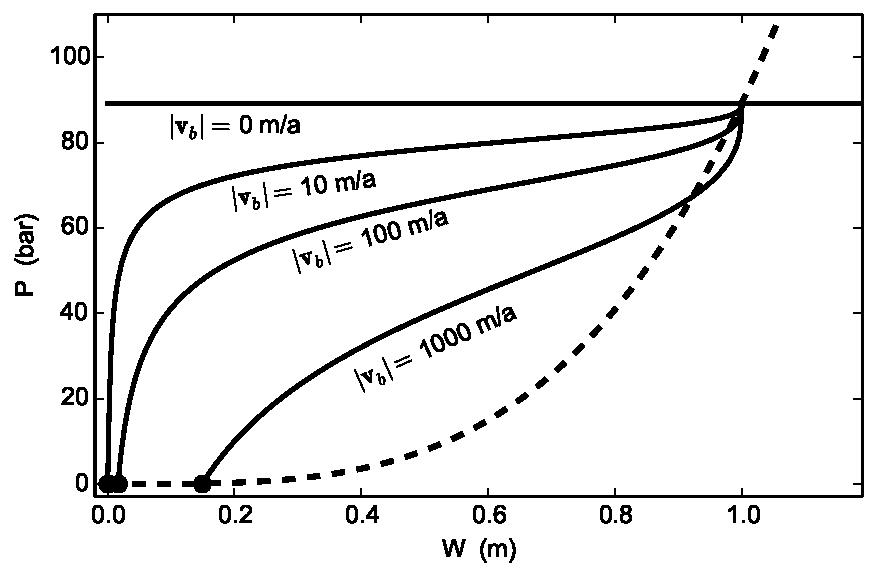
\includegraphics[width=3.0in,keepaspectratio=true]{figs/psteady-vb} \, 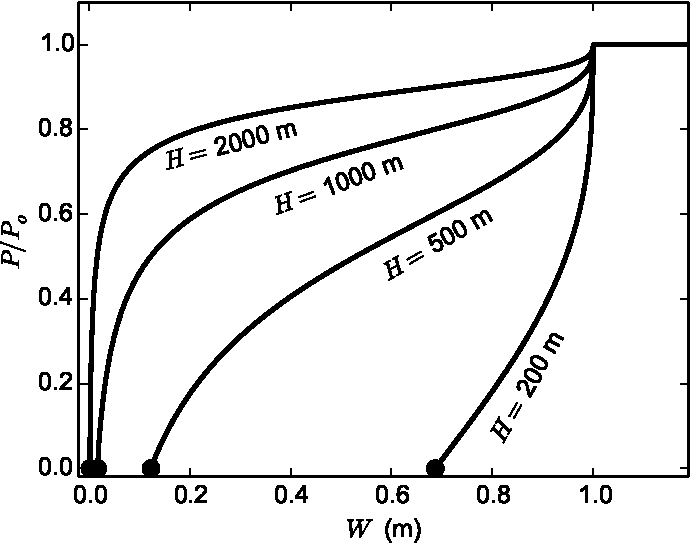
\includegraphics[width=3.0in,keepaspectratio=true]{figs/psteady-Po}
\medskip
\caption{(a) The steady state function $P(W)$ (equation \eqref{eq:PofWsteady}) depends on the sliding speed $|\bv_b|$; four cases are shown (solid curves) using a fixed uniform ice thickness of $H=1000$ m.  Relation \eqref{eq:PofWFC} is shown with $W_{\text{crit}}=0.5$ m for comparison (dashed black).  (b)  The same function $P(W)$ depends on overburden pressure $P_o=\rho_i g H$.  We fix $|\bv_b|=100$ m/a and consider four cases of uniform thickness $H$.}
\label{fig:psteady}
\end{figure}

\cite{FlowersClarke2002_theory} propose a functional relation for all conditions, steady and not steady, namely
\begin{equation}
P_{FC}(W) = P_o \left(\frac{W}{W_{\text{crit}}}\right)^{7/2}. \label{eq:PofWFC}
\end{equation}
This is used to describe the water pressure under glaciers including the Trapridge glacier in Canada.  On the one hand their formula has features in common with equation \eqref{eq:PofWsteady}: both functions are increasing and both give zero pressure at $W=0$ (at least in $|\bv_b|>0$ cases for \eqref{eq:PofWsteady}).  Also, both relate the water pressure to the overburden pressure $P_o$, but while in \eqref{eq:PofWsteady} this is additive, in \eqref{eq:PofWFC} the overburden pressure is a multiplicative scaling.  The power law form of $P_{FC}(W)$ is not, however, justified by the physical reasoning which led to equation \eqref{eq:PofWsteady}, even in steady state.  For example, it would appear that any functional relationship $P(W)$ should also depend on the sliding velocity if cavitation is an influence on the water pressure.  Furthermore the $W>W_{\text{crit}}$ case gives $P_{FC}(W) > P_o$, a physically-inconsistent state that does not arise in \eqref{eq:PofWsteady}.  The most important contrast of the \cite{FlowersClarke2002_theory} work and the current paper, however, is that we have no such functional relationship $P(W)$ in the nonsteady theory.

\subsection*{Velocity in steady state}  Equation \eqref{eq:PofWsteady} can be written
\begin{equation}
P(W) = \left(P_o - s_b \left((W_r - W)_+/W\right)^{1/3}\right)_+.  \label{eq:againPofWsteady}
\end{equation}
In calculations below we will also need the derivative formula for the variation of $P$ when holding $P_o$ and $|\bv_b|$ constant; it only applies in steady state:
\begin{equation}
\frac{\partial P}{\partial W} =
    \begin{cases}
      0, & \bv_b = 0 \text{ or } W > W_r \text{ or } P_o^3 W < s_b^3 (W_r - W), \\
      \frac{1}{3} s_b W_r (W_r - W)^{-2/3} W^{-4/3}, & \text{otherwise}.
    \end{cases}  \label{eq:dPdWsteady}
\end{equation}
The last case is the ``normal pressure'' case, where $0 < P < P_o$.  Formula \eqref{eq:dPdWsteady} also reveals that $\partial P / \partial W \to \infty$ as $W \to W_r$ or $W\to 0$ in many normal pressure cases.

Equations \eqref{eq:Vsteady}, \eqref{eq:againPofWsteady}, and \eqref{eq:dPdWsteady} yield a formula for the velocity in steady state, in the normal pressure ($0 < P < P_o$) cases:
\begin{align}
\bV &= - c_0 \left[\frac{\partial P}{\partial P_o} \grad P_o + \frac{\partial P}{\partial s_b} \grad s_b + \frac{\partial P}{\partial W} \grad W\right] - K \grad b  \notag \\
    &= - c_0 \left[\grad P_o - \left(\frac{W_r - W}{W}\right)^{1/3} \grad s_b + \frac{s_b W_r}{3 (W_r - W)^{2/3} W^{4/3}} \grad W\right] - K \grad b \notag \\
    &= - c_0 \left[\grad \psi_o - \left(\frac{W_r - W}{W}\right)^{1/3} \grad s_b + \frac{s_b W_r}{3 (W_r - W)^{2/3} W^{4/3}} \grad W\right]. \label{eq:Vsteadyexpand}
\end{align}
We have simplified the last expression by combining terms using the purely-geometrical function $\psi_o = P_o + \rho_w g b = \rho_i g H + \rho_w g b$, the \emph{overburden potential} which is the hydraulic potential associated to an infinitesimal amount of waterin the subglacial layer if it is at  zero effective pressure.

Equation \eqref{eq:Vsteadyexpand} can help us understand the advective flux
\begin{equation}
\bV W = - c_0 \left[W \grad \psi_o - W^{2/3} \left(W_r - W\right)^{1/3} \grad s_b + \frac{s_b W_r}{3 (W_r - W)^{2/3} W^{1/3}} \grad W\right].  \label{eq:qsteadyexpand}
\end{equation}
First, the direction of water transport $\bV$ is determined in steady state by a combination of a geometric direction ($\grad \psi_o$), a direction derived from variations in the sliding speed ($\grad s_b$), and a diffusive direction (i.e.~proportional to $-\grad W$).  Unsurprisingly, when the ice thickness, bed elevation, sliding velocity, or water thickness are highly variable in space then we can expect a larger amount of flow.  Because that the magnitude of the velocity $|\bV|$ determines the CFL time step restriction \citep{MortonMayers} associated to numerically solving the mass conservation equation in the model \eqref{eq:bluebox}, large variations in the same fields will generally reduce the time steps taken by our model.

The linear combination in \eqref{eq:qsteadyexpand} has coefficients which are functions of water amount $W$.  The first two coefficients, of the terms with $\grad \psi_o$ and $\grad s_b$, go to zero as $W\to 0^+$.  In this same $W\to 0^+$ limit the third flux component, the diffusive one, dominates.  Also when the water thickness closely approximates the roughness scale ($W\approx W_r$) then the second sliding term contributes little while the third diffusive term is strong.

\subsection*{A nearly-exact two-dimensional solution}  The above steady equations are the basis for building a useful two-dimensional nearly-exact solution for $W$ and $P$.  This solution will depend on a single numerical solution of a first-order ODE which can be solved to very high precision.  Exact solutions in one horizontal dimension appear in \cite{Schoofetal2012}.  Here, by contrast, we consider a two horizontal dimension ice sheet geometry on a flat bedrock.

Assume that all quantities vary only with the radial coordinate $r = \sqrt{x^2+y^2}$.  Consider steady state equations \eqref{eq:Vsteady}--\eqref{eq:masscontsteady} and eliminate $\bV$.  In the flat bed case the resulting pair of equations is
\begin{align}
q(r) &= - c_0 W(r)\, \left(P'(r) + \rho_w g W'(r)\right), \label{eq:rsflux} \\
\frac{1}{r}\left(r\,q(r)\right)' &= \Phi(r). \label{eq:rsconserve}
\end{align}
In the case of constant water input $\Phi(r)=\Phi_0$, which we assume for the exact solution, from \eqref{eq:rsconserve} we can integrate from $0$ to $r$ and use symmetry ($q(0)=0$) to get
\begin{equation}
q(r) = \frac{1}{2} \Phi_0\, r. \label{eq:qradial}
\end{equation}

On the other hand, equation \eqref{eq:againPofWsteady} gives $P$ as a function of $W$ in steady state.  Assume $W(r) < W_r$ and that the scaled sliding speed $s_b(r)$ has a bounded derivative; both of these properties must be verified later for the constructed solution.  Now, by combining \eqref{eq:rsflux}, \eqref{eq:qradial}, and \eqref{eq:againPofWsteady} we can eliminate $q$ and $P$ to find
	$$\frac{1}{2} \Phi_0\, r = - c_0 W(r)\, \left(P_o'(r) - \left[s_b(r) \left(\frac{W_r - W(r)}{W(r)}\right)^{1/3}\right]' + \rho_w g W'(r)\right).$$
This is a first-order ordinary differential equation (ODE) for $W(r)$.  To put it in the standard form expected by a numerical ODE solver, let $\varphi_0 = \Phi_0 / (2 c_0)$ and solve the equation above for $W'(r)$:
\begin{equation}
W'(r) = \frac{s_b'(r) W(r) \left(W_r - W(r)\right) - \Big[\varphi_0\, r + P_o'(r) W(r)\Big] W(r)^{1/3} \left(W_r - W(r)\right)^{2/3}}{\frac{1}{3} W_r\, s_b(r) + \rho_w g W(r)^{4/3} \left(W_r - W(r)\right)^{2/3}}.
\label{eq:WradialODE}
\end{equation}
%DONE for now:  The nontrivial manipulations needed to derive this form should be carefully checked.
Note that ODE \eqref{eq:WradialODE} has a constant solution $W(r)=W_r$.  To determine a nontrivial nearly-exact solution of this ODE we must choose an ice thickness $H(r)$ and a sliding speed $|\bv_b|(r)$.  These functions determine $P_o'(r)$ and $s_b'(r)$, respectively, in \eqref{eq:WradialODE}.  

The numerical solution of ODE \eqref{eq:WradialODE} will proceed from the ice margin inward toward the center.  In fact, by applying equation \eqref{eq:openclosesteady} at the ice margin, where $P_o(r)\to 0$ and $P(r)\to 0$ thus because $0 \le P \le P_o$, we see that $W(r)\to W_r$ at the margin.  (This applies in the case $W(r)\le W_r$ which will be true for our nearly-exact solution.)  If $r=R_0$ is the position of the margin then $W(R_0)=W_r$ is the initial condition for solving \eqref{eq:WradialODE}.  We integrate the ODE from $r=R_0$ to $r=0$.  The central value $W(0)$ is determined as part of the solution.

We need an ice cap geometry $h(r)$ in which the surface gradient is bounded so that $P_o'(r)$ in \eqref{eq:WradialODE} is bounded.  The plug flow, flat bed solution of \cite{Bodvardsson} has this property.  Extending to the radial case, equations (23) and (24) of \citep{Bodvardsson} give
\begin{equation}
h(r) = h_0 \left(1 - \frac{r^2}{R_0^2} \right) \label{eq:choosebodvardssonh}
\end{equation}
where $h(0)=h_0$ is the height of the center of the ice cap (Figure \ref{fig:h-vb}).  It follows that $P_o'(r) = - C r$ where $C=2\rho_i g h_0 R_0^{-2}$.

The sliding speed could potentially be determined by a model for stresses at the ice base and within the ice \citep{Bodvardsson,GreveBlatter2009}, but this kind of coupled ice and water dynamics solution is too advanced for the current purpose of decoupled model verification.  Instead we choose a well-behaved sliding speed function to see how it affects the current model.  It has no sliding near the ice cap center, and increasing sliding near the margin:
\begin{equation}
|\bv_b|(r) = \begin{cases} 0, & 0 \le r \le R_1, \\
                           v_0  \left(\frac{r-R_1}{R_0-R_1}\right)^5, & R_1 < r < R_0, \\
                           0, & R_0 \le r.
             \end{cases}  \label{eq:choosevb}
\end{equation}
(See figure \ref{fig:h-vb}.)  It follows that where there is sliding (i.e.~$R_1 < r < R_0$) we have
\begin{equation}
s_b'(r) = - \frac{5 \tilde C}{3 (R_0-R_1)} \left(\frac{r-R_1}{R_0-R_1}\right)^{2/3}, \label{eq:determinessbprime}
\end{equation}
where $\tilde C = (c_1 v_0/(c_2 A))^{1/3}$, which is continuous at $r=R_1$ and bounded on $0\le r \le R_0$.

\begin{figure}[ht]
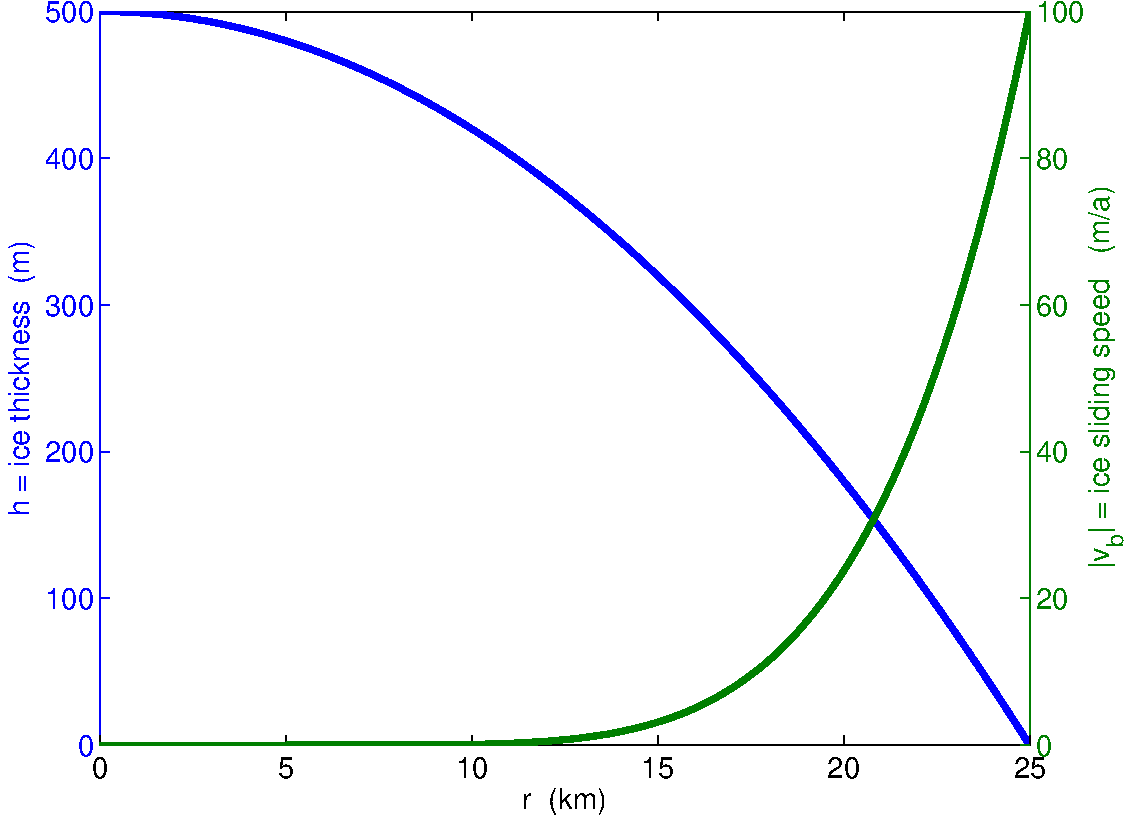
\includegraphics[width=3.0in,keepaspectratio=true]{figs/h-vb-plot}
\caption{Surface elevation $h(r)$ and sliding speed $|\bv_b|(r)$ for flat bed, radial, steady state, nearly-exact solution.}
\label{fig:h-vb}
\end{figure}



FIXME: comment on exact $W(r)$ and $P(r)$

\begin{figure}[ht]
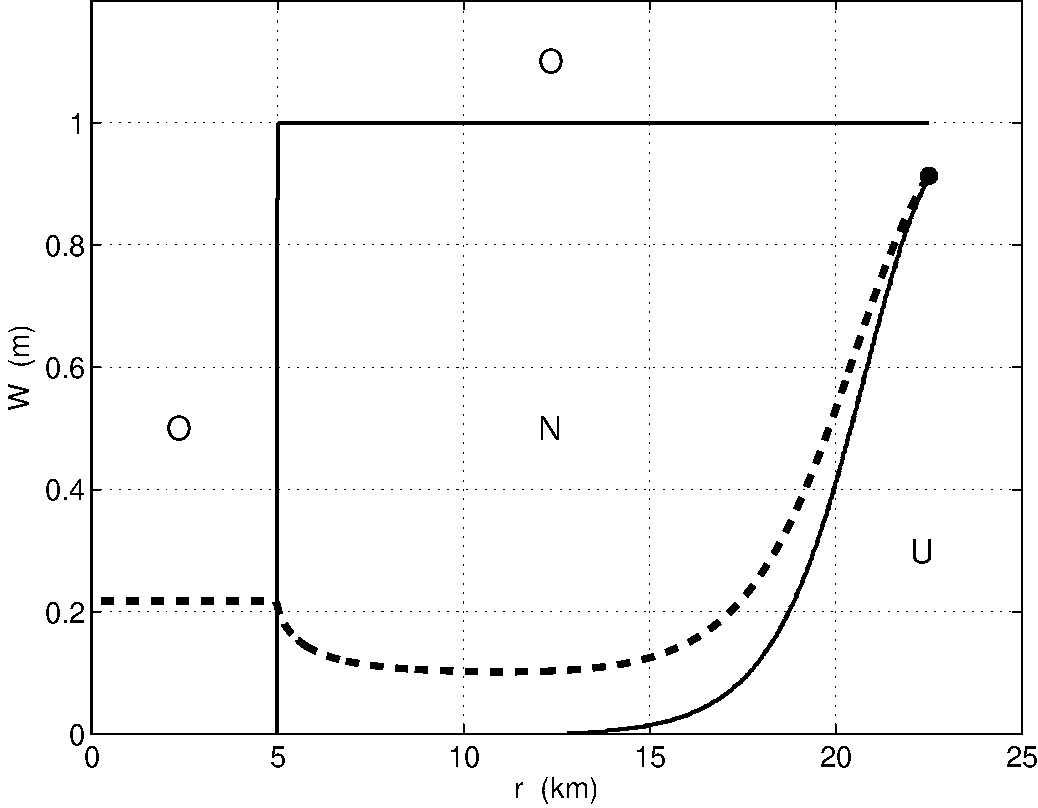
\includegraphics[height=2.3in,keepaspectratio=true]{figs/exact-W-plot-onu} \, 
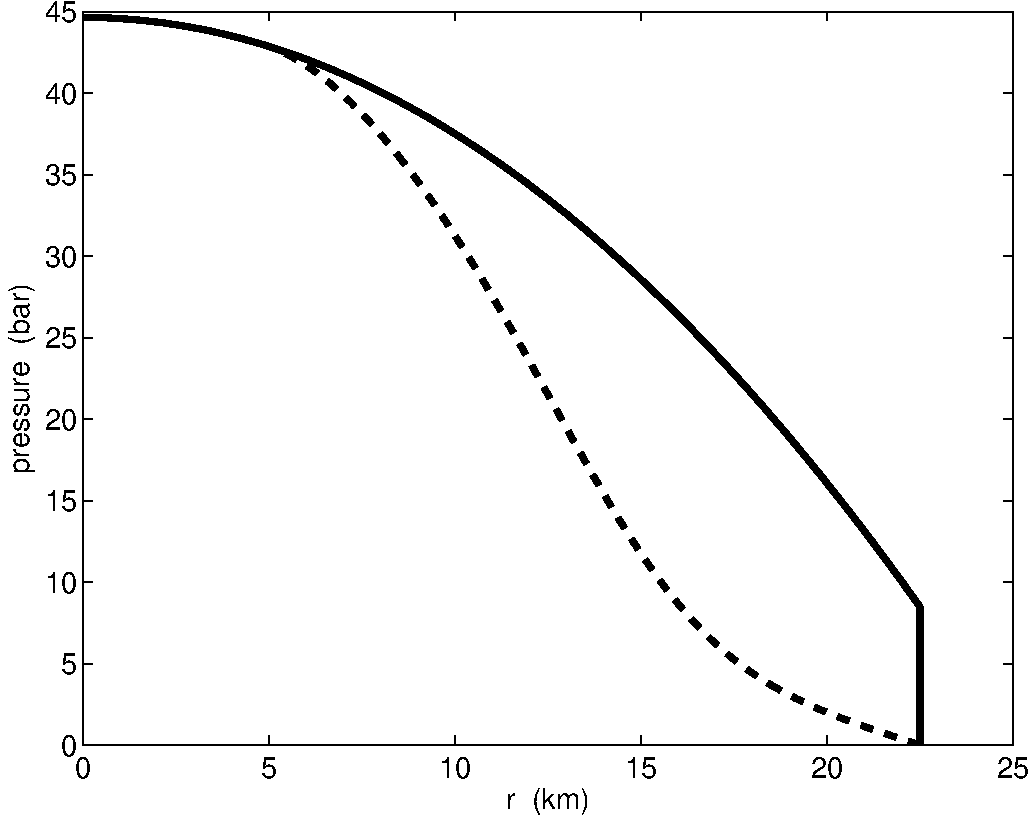
\includegraphics[height=2.33in,keepaspectratio=true]{figs/exact-P-plot}
\caption{Nearly-exact solutions for water thickness $W(r)$ (left; dashed) and pressure $P(r)$ (right; dashed) for radial, steady state exact solution.  In $r$-versus-$W$ space the the overpressure (O), normal pressure (N), and underpressure (U) regions are determined (left; solid).}
\label{fig:WPexact}
\end{figure}


\begin{table}[ht]
  \centering
  \caption{Constants used in constructing the nearly-exact solution.}
  \begin{tabular}{lllp{3.0in}}
    \textbf{Name} & \textbf{Value} & \textbf{Units} & \textbf{Description}\\
\hline
    $\Phi_0$ & $20$ & $\text{cm}\,\text{a}^{-1}$ & water input rate \\
    $h_0$ & $500$ & m & ice cap center thickness \\
    $R_0$ & $25$  & km & ice cap radius \\
    $R_1$ & $5$   & km & radial location $r=R_1$ of onset of sliding \\
    $v_0$ & $100$ & $\text{m}\,\text{s}^{-1}$ & sliding speed scale \\
    \hline
  \end{tabular}
 \label{tab:verifconstants}
\end{table}

\section{Numerical scheme}  \label{sec:num}

\subsection*{Numerical scheme for the mass conservation equation}  The mass conservation equation \eqref{eq:adeqn} will be discretized by an explicit conservative first-order upwind method for the advection part and an explicit centered, second-order scheme for the nonlinear diffusion part.  We consider stable time steps for this scheme immediately.  The time step restriction for the advective part, i.e.~the CFL condition on the upwind scheme, is much more restrictive than the time-step restriction for the diffusion in \eqref{eq:adeqn}.  In fact, in the Appendix it is shown that for stability the time step should satisfy $\Delta t \le \Delta t_{\text{CFL}}$ where
\begin{equation}
\Delta t_{\text{CFL}} \left(\frac{\max |\alpha|}{\Delta x} + \frac{\max |\beta|}{\Delta y}\right) = \frac{1}{2}. \label{eq:dtCFL}
\end{equation}
Here $V=(\alpha,\beta)$ is the advection velocity, for the upwind part of the scheme to maintain stability.  Because of the diffusion part, the time step should also satisfy $\Delta t \le \Delta t_{W}$ where
\begin{equation}
\Delta t_W\, (2 K \max W) \left(\frac{1}{\Delta x^2} + \frac{1}{\Delta y^2}\right) = \frac{1}{2} \label{eq:dtDIFFW}
\end{equation}
for the diffusion scheme to be stable.

To understand the significance of these time step restrictions, we consider typical values of the parameters.  We are interested in grids of size $\Delta x = \Delta y = 500$ m or larger.  The maximum water speed $|\bV|$ is about $10^5$ m/a in trial runs of the model, so $\max |\alpha| = \max |\beta| \approx 0.002$ m/s.  (There is significant uncertainty in estimating such velocities, which are part of the solutions to the model, not data provided to it.)  We take $K=10^{-2}$ m/s and $\max W=1$ m as representative values.  With these values the advective restriction \eqref{eq:dtCFL} gives $\Delta t_{\text{CFL}} \approx 0.001$ year while the diffusive restriction from \eqref{eq:dtDIFFW} is $\Delta t_W \approx 0.1$ year.  Thus, unless velocities are unusually slow, or unless deep subglacial lakes develop so that $KW$ is large and $\Delta t_W$ is correspondingly small, we should not worry so much about this diffusive time scale.

To explain the upwind method for \eqref{eq:adeqn}, consider the model equation
\begin{equation} \label{eq:modeladvect}
u_t + (v(x) u)_x = 0
\end{equation}
for some quantity $u(t,x)$ transported by a flux $q = v(x) u$.  A ``donor cell'' upwind scheme can be described as a finite volume scheme \citep{LeVeque} wherein a grid point $x_j$ is the center of a cell.  We consider the flux at the cell interfaces $x_{j-1/2}$ and $x_{j+1/2}$.  We decide which cell contributes the advected quantity $U$ based on the sign of the velocity $v(x)$ at these interfaces.

The scheme is easier to display if we define the following upwind notation,
\newcommand{\up}[2]{\big<#1\big|\,#2\big>}
	$$\up{v}{U_j} := v \begin{Bmatrix} U_j, & v \ge 0 \\ U_{j+1}, & v < 0 \end{Bmatrix}.$$
For the model equation \eqref{eq:modeladvect} on a space-time grid $(t_l,x_j)$ we set
\begin{equation}\label{eq:modelfdadvect}
\frac{U_j^{l+1} - U_j^l}{\Delta t} + \frac{\up{v_+}{U_j^l} - \up{v_-}{U_{j-1}^l}}{\Delta x} = 0
\end{equation}
where $v_+ = v(x_{j+1/2})$ and $v_-=v(x_{j-1/2})$.

\begin{figure}[ht]
\centering
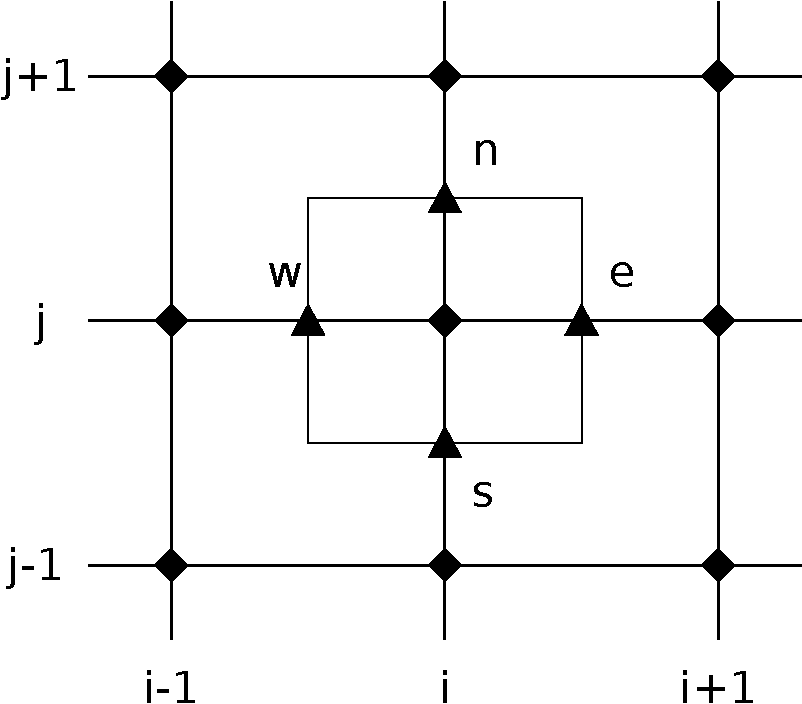
\includegraphics[width=2.5in,keepaspectratio=true]{figs/diffstencil}
\bigskip
\caption{Numerical scheme \eqref{eq:Wfd} for Equation \eqref{eq:adeqn} is a finite volume scheme for the grid-centered cell (dashed line).  The velocity and diffusivity are evaluated at the staggered grid locations (triangles).  The state functions $W,P$ live at the regular grid points (diamonds).}
\label{fig:stencil}
\end{figure}

Now we can state our scheme for equation \eqref{eq:adeqn}.  To set notation, suppose our rectangular computational domain has $M_x \times M_y$ gridpoints $(x_i,y_j)$ with uniform spacing $\Delta x,\Delta y$.  Let $\Wlij \approx W(t_l,x_i,y_j)$ and $\Plij \approx P(t_l,x_i,y_j)$ be the approximations of the continuum solution at the grid points.  Recall that $\bV = - c_0 \grad P - K \grad b$ and $\Div \left(\bV W\right) = (\alpha W)_x + (\beta W)_y$.  We will compute velocity components at staggered (cell-face-centered) points as in Figure \ref{fig:stencil}.  We compute these values based on centered finite difference approximations of Equation \eqref{eq:vexpression}.  We use ``compass'' notation like $\alpha_e = \alpha_{i+1/2,j}$, and so on, for the components:
\begin{align}
\alpha_e &= - c_0 \frac{P_{i+1,j}-P_{i,j}}{\Delta x} - K \frac{b_{i+1,j}-b_{i,j}}{\Delta x}, \qquad \alpha_w = - c_0 \frac{P_{i,j}-P_{i-1,j}}{\Delta x} - K \frac{b_{i,j}-b_{i-1,j}}{\Delta x}, \label{eq:velocitycomp} \\
\beta_n  &= - c_0 \frac{P_{i,j+1}-P_{i,j}}{\Delta y} - K \frac{b_{i,j+1}-b_{i,j}}{\Delta y}, \qquad \beta_s = - c_0 \frac{P_{i,j}-P_{i,j-1}}{\Delta y} - K \frac{b_{i,j}-b_{i,j-1}}{\Delta y}. \notag
\end{align}
For the diffusive term the staggered-grid values are computed by averaging:
\begin{align}
W_e &= (W_{i,j}^l + W_{i+1,j}^l)/2, & W_w &= (W_{i-1,j}^l + W_{i,j}^l)/2, \label{eq:stagW} \\
W_n &= (W_{i,j}^l + W_{i,j+1}^l)/2, & W_s &= (W_{i,j-1}^l + W_{i,j}^l)/2. \notag
\end{align}
We apply the conservative upwind scheme in each variable, indicating the active index (either $i$ or $j$) in our upwind notation:
\begin{align}
 &\frac{W_{i,j}^{l+1} - \Wlij}{\Delta t} + \frac{\upp{\alpha_e}{\Wlij}{i} - \upp{\alpha_w}{W_{i-1,j}^l}{i}}{\Delta x} + \frac{\upp{\beta_n}{\Wlij}{j} - \upp{\beta_s}{W_{i,j-1}^l}{j}}{\Delta y}  \label{eq:Wfd} \\
      &\qquad = K \bigg[\frac{W_e \left(W_{i+1,j}^l - \Wlij\right) - W_w \left(\Wlij - W_{i-1,j}^l\right)}{\Delta x^2}  \notag \\
      &\qquad\qquad\qquad + \frac{W_n \left(W_{i,j+1}^l - \Wlij\right) - W_s \left(\Wlij - W_{i,j-1}^l\right)}{\Delta y^2}\bigg] + \Phi_{ij}. \notag
\end{align}
This scheme, which uses first-order upwinding, has $O(\Delta t^1 + \Delta x^1 + \Delta y^1)$ truncation error.

Because of the positivity proven in the appendix for this scheme, if $\Phi\ge 0$ then the lower bound $W\ge 0$ is true for the updated values at the new time $t_{l+1}$ if it is true at time $t_l$.  However, because refreeze is possible, generally $\Phi$ has either sign and so we must enforce $W\ge 0$ on the updated values.

\subsection*{Numerical scheme for the pressure evolution equation}  The pressure evolution equation \eqref{eq:diffusionpressure} is a nonlinear diffusion with additional ``reaction'' terms associated to opening and closing.  Unlike \eqref{eq:adeqn} there is no dominating advection term.  We discretize it using an explicit centered, second-order scheme.  Again, because this is an explicit scheme, we consider stable time steps immediately.

The time step restriction is comparable to \eqref{eq:dtDIFFW}, though the proof in the appendix does not suffice to \emph{prove} stability under this condition because of the additional reaction terms.  Noting that $P_o=\rho_i g H$, the time step must satisfy $\Delta t \le \Delta t_P$ where
\begin{equation}
\Delta t_P\, \left(\frac{2 K \rho_i \max H \max W}{\rho_w E_0}\right) \left(\frac{1}{\Delta x^2} + \frac{1}{\Delta y^2}\right) = \frac{1}{2} \label{eq:dtDIFFP}
\end{equation}

The resulting time step $\Delta t_P$ is a fraction of $\Delta t_W$ from \eqref{eq:dtDIFFW}:
\begin{equation}
\Delta t_P = \frac{\rho_w E_0}{\rho_i \max H}\, \Delta t_W.
\end{equation}
In fact, with the estimates $\rho_w/\rho_i \approx 1$, $E_0\approx 1$ m, and $\max H \approx 1000$ m we have $\Delta t_P$ which is about 1000 times smaller than $\Delta t_W$.  With these values and others used earlier (i.e.~$\Delta x = \Delta y = 500$ m, $\max |\bV|=10^5$ m/a, $K=10^{-2}$ m/s and $\max W=1$ m) we get
\begin{align*}
  \Delta t_{\text{CFL}} &\approx 0.001  \text{ year} &&\text{ from \eqref{eq:dtCFL}}, \\
  \Delta t_W            &\approx 0.1    \text{ year} &&\text{ from \eqref{eq:dtDIFFW}}, \\
  \Delta t_P            &\approx 0.0001 \text{ year} &&\text{ from \eqref{eq:dtDIFFP}.}
\end{align*}
Thus the numerical scheme for pressure diffusion, given next, has the shortest time step.  This analysis says if is only about 10 times shorter than the CFL restriction for the advection, however.  Furthermore, the precise size of the stable time step $\Delta t_P$ scales inversely with the adjustable small thickness $E_0$.  By choosing $E_0$ larger or smaller we can make the time step restriction on $\Delta t_P$ less or more severe, respectively.

Now, the scheme we use for \eqref{eq:diffusionpressure} is similar to \eqref{eq:Wfd} for \eqref{eq:adeqn} but without a need for approximating advection:
\begin{align}
\frac{E_0}{(P_o)_{i,j}} \frac{P_{i,j}^{l+1} - \Plij}{\Delta t} &= c_0 \bigg[\frac{W_e \left(\psi_{i+1,j}^l - \psi_{i,j}^l\right) - W_w \left(\psi_{i,j}^l - \psi_{i-1,j}^l\right)}{\Delta x^2}  \label{eq:Pfd} \\
      &\qquad\qquad + \frac{W_n \left(\psi_{i,j+1}^l - \psi_{i,j}^l\right) - W_s \left(\psi_{i,j}^l - \psi_{i,j-1}^l\right)}{\Delta y^2}\bigg] \notag \\
      &\qquad + c_2 A \left(\rho_i g H_{i,j}- \Plij\right)^3 \Wlij - c_1 |\bv_b|_{i,j} \left(W_r - \Wlij\right)_+ + \Phi_{i,j}. \notag
\end{align}
For implementation it is useful to restate \eqref{eq:Pfd} in explicit update form.  First define
	$$\omega_x = \frac{c_0 \Delta t}{\Delta x^2}, \qquad \omega_y = \frac{c_0 \Delta t}{\Delta y^2}.$$
Also let
\newcommand{\Ocavij}{O_{\text{cav};\, i,j}}
\newcommand{\Ccrpij}{C_{\text{crp};\, i,j}}
	$$\Ocavij = c_1 |\bv_b|_{i,j} \left(W_r - \Wlij\right)_+, \qquad \Ccrpij = c_2 A \left(\rho_i g H_{i,j} - \Plij\right)^3 \Wlij$$
be the gridded values of the cavitation-opening and creep-closure rates.  Then scheme \eqref{eq:Pfd} is equivalent to this form:
\begin{align}
P_{i,j}^{l+1} &= \Plij +  \frac{(P_o)_{i,j}}{E_0} \bigg[\omega_x W_e \left(\psi_{i+1,j}^l - \psi_{i,j}^l\right) - \omega_x W_w \left(\psi_{i,j}^l - \psi_{i-1,j}^l\right) \label{eq:Pfdupdate} \\
      &\qquad\qquad\qquad\quad + \omega_y W_n \left(\psi_{i,j+1}^l - \psi_{i,j}^l\right) - \omega_y W_s \left(\psi_{i,j}^l - \psi_{i,j-1}^l\right) \notag \\
      &\qquad\qquad\qquad\quad + \Delta t\, \left(\Ccrpij - \Ocavij + \Phi_{i,j}\right)\bigg]. \notag
\end{align}

\subsection*{One time step of the model}  Mathematical model \eqref{eq:bluebox} evolves $W$ and $P$.  One time step of this evolution is described as follows.

Assume geometry fixed and thus $h_{i,j}$, $b_{i,j}$ and $(P_o)_{i,j}$ are determined for the duration of the run.  We start the step with values $\Wlij$, $\Plij$ which satisfy the bounds $W\ge 0$ and $0 \le P \le P_o$.  Get velocity components at staggered grid locations from \eqref{eq:velocitycomp}.  Get $W$ values averaged onto the staggered grid from \eqref{eq:stagW}.  Compute the current values of the hydraulic potential, $\psi_{i,j}^l = \Plij + \rho_w g(b_{i,j} + \Wlij)$.  Use \eqref{eq:Wfd} and \eqref{eq:Pfdupdate} to compute preliminary values for $W_{i,j}^{l+1}$ and $P_{i,j}^{l+1}$.

Generally $\Phi$ has either sign and so we must enforce $W\ge 0$ on the updated values, that is, we project.  Thus, if $W_{i,j}^{l+1}<0$ at the end of a step we reset $W_{i,j}^{l+1}=0$.  The amount of mass created by this projection should be accounted for.  As the temporal grid is refined, however, this mass conservation error should decrease.  Alternatively we could redistribute mass to preserve exact conservation.

There is no expectation that pressure update \eqref{eq:Pfdupdate} will preserve our bounds $0\le P \le P_o$.  Thus, at the end of each pressure-update time step we also project to put the pressure $P_{i,j}^{l+1}$ back into the correct range.  However, because the pressure is not a conserved quantity, this projection step does not suggest an attempt to redistribute pressure.

FIXME: icefree land gets $W=0$ and $P=0$.  the base of floating ice gets $W=0$ and $P=P_o$.  the water lost by these mechanisms is what is produced by the model.

\small
\bibliography{ice_bib}  % generally requires link to pism/doc/ice_bib.bib
\bibliographystyle{agu}
\normalsize

\appendix

\section{Positivity and stability of the mass conservation scheme}

Explicit numerical scheme \eqref{eq:Wfd} for the model PDE \eqref{eq:adeqn} is sufficiently simple so that we can analyze its properties.  The scheme is conditionally stable as we now show.  In fact, in this appendix we sketch a maximum principle argument \citep{MortonMayers} which shows both stability and this positivity-preserving property: if the water input $\Phi$ is nonnegative and the discrete water thicknesses $\Wlij$ are nonnegative then, under the given stability conditions, the updated values $W_{i,j}^{l+1}$ are also nonnegative.    We consider only the case where all of the discrete velocities at the centers of cell interfaces are nonnegative: $\alpha_e\ge 0$, $\alpha_w\ge 0$, $\beta_n\ge 0$, $\beta_s\ge 0$.  The many other upwinding cases, wherein these velocity components have various signs, can be handled by similar special-case arguments like the present one; they are an exercise for the reader.

Let $\nu_x = \Delta t/\Delta x$, $\nu_y = \Delta t/\Delta y$, $\mu_x = K \Delta t / (\Delta x)^2$, and $\mu_y = K \Delta t / (\Delta y)^2$.  We rewrite \eqref{eq:Wfd} as a computation of the next value $W_{i,j}^{l+1}$, and collect terms:
\begin{align*}
 W_{i,j}^{l+1} &= \Wlij - \nu_x \left(\alpha_e \Wlij - \alpha_w W_{i-1,j}^l\right) - \nu_y \left(\beta_n \Wlij - \beta_s W_{i,j-1}^l\right)  \\
      &\qquad + \mu_x \left[W_e \left(W_{i+1,j}^l - \Wlij\right) - W_w \left(\Wlij - W_{i-1,j}^l\right)\right]  \\
      &\qquad + \mu_y \left[W_n \left(W_{i,j+1}^l - \Wlij\right) - W_s \left(\Wlij - W_{i,j-1}^l\right)\right] + \Delta t \Phi_{ij}.
\end{align*}
Rearranging a bit further we get
\begin{align*}
 W_{i,j}^{l+1} &= (\nu_x \alpha_w + \mu_x W_w) W_{i-1,j}^l + (\mu_x W_e) W_{i+1,j}^l + (\nu_y \beta_s + \mu_y W_s) W_{i,j-1}^l + (\mu_y W_n) W_{i,j+1}^l \\
      &\qquad + \Big[1 - \nu_x \alpha_e - \nu_y \beta_n - \mu_x (W_e + W_w) - \mu_y (W_n + W_s)\Big] \Wlij + \Delta t \Phi_{ij}
\end{align*}
so that the new value is a linear combination of the old values, plus a source term:
\begin{equation}
W_{i,j}^{l+1} = A W_{i-1,j}^l + B W_{i+1,j}^l + C W_{i,j-1}^l + D W_{i,j+1}^l + E \Wlij + \Delta t \Phi_{ij}. \label{eq:lincomb}
\end{equation}
Because of our assumption about nonnegative velocities, and assuming $\Wlij \ge 0$ for all $i,j$, we see that coefficients $A,B,C,D$ are all nonnegative, and that only $E$ could be negative.  Thus we can state a sufficient condition based on an equal split between advective and diffusive parts.  First assume a CFL-type time step restriction for the advection term in  \eqref{eq:adeqn}:
\begin{equation}
\nu_x \alpha_e + \nu_y \beta_n = \Delta t \left(\frac{\alpha_e}{\Delta x} + \frac{\beta_n}{\Delta y}\right) \le \frac{1}{2}. \label{eq:adstabcond}
\end{equation}
Also assume a second time-step restriction on the diffusion:
\begin{equation}
\mu_x (W_e + W_w) + \mu_y (W_n + W_s) = \Delta t \left(\frac{K(W_e + W_w)}{\Delta x^2} + \frac{K(W_n + W_s)}{\Delta y^2}\right) \le \frac{1}{2}. \label{eq:diffstabcond}
\end{equation}
The right-hand sides of these inequalities are each $1/2$, and of course $1-(1/2)-(1/2)=0$.  Thus the coefficient $E$ in \eqref{eq:lincomb} is nonnegative:
	$$E = 1 - \nu_x \alpha_e - \nu_y \beta_n - \mu_x (W_e + W_w) - \mu_y (W_n + W_s) \ge 0.$$
It follows from \eqref{eq:lincomb} that if $\Wlij\ge 0$ and $\Phi_{ij}\ge 0$ for all $i,j$ then $W_{ij}^{l+1}\ge 0$.

Though the argument above can only be made fully rigorous by handling all upwind cases (not shown), we see that all coefficients in linear combination \eqref{eq:lincomb} are nonnegative if the time step restrictions are satisfied.  Furthermore the coefficients add to one.  It follows \citep{MortonMayers} that scheme \eqref{eq:Wfd} is positivity-preserving when $\Phi\ge 0$.  It also follows that the scheme is stable under conditions \eqref{eq:dtCFL} and \eqref{eq:dtDIFFW}, the all-upwinding-cases generalizations of inequalities \eqref{eq:adstabcond} and \eqref{eq:diffstabcond}, respectively.


\end{document}
